\chapter{Introdução}
\label{introducao}

O ser humano vem usando a sua habilidade de reconhecimento de padrões desde  muito antes do início do processo civilizatório. Grupos de humanos paleolíticos já faziam registro dos padrões migratórios de certos grupos de cervídeos. Durante a aurora da revolução neolítica, nossa capacidade de reconhecimento de padrões foi direcionada para a agricultura com a criação de monumentos que registraram a mudança das estações ao longo do ano.

O cérebro humano evoluiu espantosamente. E no que se refere a quantidade de informação processada, o cérebro possui enorme vantagem em relação a quantidade de informação processada por um computador \citep{Hall2014}. Este não para de funcionar somente porque algumas células morrem. Um computador, por sua vez, não funciona quando há degradação da sua unidade central de processamento \citep{Mao1996}.

O campo do aprendizado de máquina aborda a criação de programas computacionais que automaticamente melhorem a si mesmos através da experiência \citep{Michie1994,Levy1997,MacKay2005}. 

%Tanto a rede neuronal quanto a árvore de decisão despontam como estratégias de solução para a resolução de problemas de reconhecimento de padrões \citep{MacKay2005}.

As Redes Neuronais Artificiais (RNA) são inspiradas em modelos sensoriais do processamento de tarefas realizadas pelo cérebro \citep{Hagan1996}. Uma RNA, portanto pode ser criada através da aplicação de algoritmos matemáticos que imitem a tarefa realizada por um neurônio \citep{Nedjah2016}. Uma rede neuronal artificial possui semelhanças com a rede neuronal \footnote{ Em muitas referências na área  da inteligência artificial usa-se o termo neural ao invés de neuronal, contudo empregar o termo neuronal é um cuidado necessário e deve ser empregado no lugar do termo neural. Isso se deve ao fato de que os primeiros modelos matemáticos foram inspirados nas células e processos presentes no sistema nervoso central e não no sistema em toda a sua completude.  } natural presente no sistema nervoso central, neste o cômputo de informações realizado do cérebro é feito através de uma vasta quantidade de neurônios interconectados \citep{Feldman1988,Poulton2002}. A comunicação entre essas células é realizada através de impulsos elétricos. Estes são transmitidos e recebidos por meio de sinapses nervosas entre axônios e dendritos. As sinapses são estruturas elementares e uma unidade funcional localizada entre dois neurônios \citep{Krogh2008}. 

%Já a árvore de decisão auxilia na predição da classe de um objeto em um estudo com base em um treinamento prévio. Ou seja, funciona como um algoritmo de aprendizado de máquina supervisionado que é basicamente aplicado em problemas de classificação \citep{FreundYoav1999}. Funciona tanto para variáveis categóricas quando para variáveis dependentes. Nesse algoritmo, a população original é dividida em dois ou mais grupos de populações homogêneas \citep{Simard2000}. 

Assim como as redes neuronais as medidas de similaridade são utilizadas como auxiliadores na predição da classe de um objeto. Ou, seja funciona como um algoritmo de aprendizado de máquina supervisionado que é basicamente aplicado em problemas de classificação\citep{FreundYoav1999}. A abordagem dos problemas de classificação sob a ótica de medidas de semelhança é um dos tópicos mais ativos dentro da área de aprendizado de máquina. O problema consiste em atribuir um rótulo a algum objeto baseado em um conjunto de atributos extraídos do mesmo. Para tal faz-se necessário, um conjunto de dados de treinamento com instâncias nal qual os rótulos dos objetos são conhecidos. 

\section{Redes Neuronais Artificiais}

\citet{McCulloch1943} redigem o trabalho pioneiro onde foi modelado um neurônio cuja resposta dependia do \textit{input}\footnote{Valor de entrada} que provinha de outros neurônios e do peso utilizado.  Já \citet{Rosenblatt1962} cria a teoria de convergência do \textit{Perceptron} onde ele prova que modelos de neurônios possuem propriedades similares ao cérebro humano \citep{Kanal2001}. Neste sentido as rede neuronais artificiais podem realizar performasses sofisticadas no reconhecimento de padrões, mesmo se alguns neurônios forem destruídos \citep{Levy1997}. \citet{Minsky1969} demonstraram que \textit{Perceptrons} somente resolvem uma classe muito limitada de problemas que podem ser linearizados.

Os primeiros artigos sobre redes neuronais em geofísica datam de $1989$ e são focalizados basicamente na eficiência da RNA diante de dados distintos e como preparar esse dado para inserí-lo na RNA e posteriormente interpretá-lo. As redes neuronais artificiais foram usualmente treinadas com dados sintéticos e depois testados em dados reais. Contudo, hoje é comum usar dados reais para treinar a rede \citep{Adibifard2014}. Embora, ambas as abordagens sejam aceitas. O foco a partir de $1995$ até o presente relaciona-se a algumas aplicações específicas, tais como caracterização de reservatórios e na integração de dados associado a uma interpretação compreensiva, ao contrário de uma aplicação isolada \citep{Poulton2002}. 

No problema específicos de poços, um passo importante é a identificação de topo e base de camadas que podem ser associadas com mudanças das propriedades petrofísicas \citep{Saljooghi2014}. Algoritmos baseados em derivadas nas curvas de log não identificam camadas muito finas, ou ruído \citep{Zhang1999}. \citet{Chakravarthy1999} consegue através do uso da função radial localizar os limites de camadas em alta definição em dados de log de indução (HDIL). Já \citet{Benaouda1999} consegue classificar tipos litológicos em poços parcialmente desmoronados através do uso da rede neuronal com propagação de erro e mudanças de classes a medida que prossegue a análise. \citet{Gloaguen2017} levanta a questão da importância relativa das propriedades físicas, em dados de perfilagem de poços,  para a tomada de decisão da rede neuronal.

O neurônio de \citet{McCulloch1943} propõe um limite binário para a criação de um modelo. Este neurônio artificial registra uma soma de pesos de $n$ sinais de entrada, $x_{j}$, $j=1,2,3,...,n$, e fornece um \textit{output}\footnote{Valor de saída} de $1$ caso esta soma esteja acima do limite $u$. Caso contrário o \textit{output} é $0$. Matematicamente essa relação pode ser descrita de acordo com a Eq. \ref{Eq.neuronio-McCulloch}:

\begin{eqnarray}
y=\theta \left( \sum^{n}_{j=1} w_{j} x_{j} -u \right)
\label{Eq.neuronio-McCulloch}
\end{eqnarray}

Onde $\theta$ é o passo dado na posição $0$, $w_{j}$ é chamada sinapse-peso associado a um $j_{esimo}$ \textit{input}. A título de simplificação a função limite\footnote{Genericamente chamada de função de ativação} $u$ é considerada um outro peso $w_{0}=-u$ anexado a um neurônio com um \textit{input} constante $x_{0}=1$. Pesos positivos correspondem a uma sinapse \textbf{excitatória}, enquanto pesos negativos correspondem a uma sinapse \textbf{inibitória}. Este modelo contém uma série de simplificações que não refletem o verdadeiro comportamento dos neurônios biológicos \citep{Mao1996}.  

Derivações do neurônio de \citet{McCulloch1943} na escolha das funções de ativação. Uma função largamente utilizada é a função sigmóide, que exibe uma suavização dos \textit{outputs} a medida que o valor da função diminui \citep{Mao1996,Misra2010}. Essa função de ativação pode ser expressa de acordo com a Eq. \ref{f.sigmoide}:

\begin{eqnarray}
g(x)=1/(1+e^{-\beta x})
\label{f.sigmoide}
\end{eqnarray}

Onde $\beta$ é o parâmetro de inclinação. A Fig. \ref{Esquematico de McCulloch} ilustra a sequência lógica da operação de uma RNA para um neurônio simples de McCulloch-Pitts. 
\\
\begin{figure}[H]
	\centering
	\setlength{\fboxsep}{8pt}
	\setlength{\fboxrule}{0.1pt}
	\fbox{
	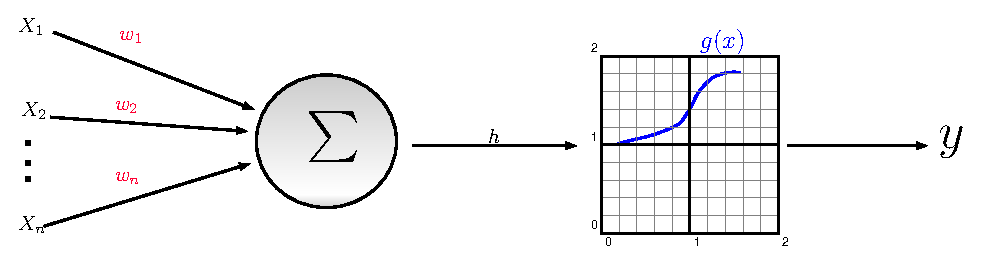
\includegraphics[scale=0.7]{Imagens/McCulloch.eps}
	}
	\caption{Modelo esquemático de um neurônio de McCulloch-Pitts. Onde $x_{1}, x_{2}, ..., x_{n}$ são os \textit{inputs}, $w_{1}, w_{2}, ..., w_{n}$ são os pesos, h é o treino, $g(x)$ é a função de ativação, e $y$ é o \textit{output}.}
	\label{Esquematico de McCulloch}
\end{figure}

Mais de $50$ tipos de redes neuronais artificiais tem sido criadas até o ano de $2014$ \citep{Saljooghi2014}.


\section{A Rede de Kohonen}

Neste trabalho, foi utilizada a rede de kohonen. Esta rede neuronal tem como importante característica ser uma rede com aprendizado não-supervisionado, portanto o espaço solução de saída da rede não é conhecido. 

A localização espacial de um neurônio da saída em um mapa topológico
corresponde a um domínio ou característica particular do dado retirado do espaço de entrada. E estas entradas são mapeadas de forma ordenada, a exemplo dos mapas cito-arqueturais do córtex cerebral.

Neste processo de identificação de padrões a redundância torna-se impreterível,
pois o neurônio da camada de saída que apresentar a maior resposta terá os seus
pesos ajustados. Além disso, o peso dos neurônios vizinhos também serão
ajustados em menor intensidade ao comparados com o neurônio vencedor.

Isto implica que os neurônios devem estar posicionados em um arranjo geométrico
adequado. Esta teoria é baseada na suposição de que as células nervosas
corticais estão organizadas anatomicamente em relação aos estímulos que recebem
dos sensores aos quais estão ligadas \citep{Artero2009}.

Este modelo exige a definição de vizinhança entre neurônios de forma geométrica. Alguns arranjos são comumente utilizados, como por exemplo, os arranjos triangulares, hexagonal, retangulares, etc.

No caso de arranjos retangulares, diferentes vizinhanças de um neurônio
$N_{i,j}$ podem ser configuradas em quartetos, diagonais e octetos. 

A Fig. \ref{hiperplano} ilustra o arranjo retangular e as vizinhanças, em quartetos, adotado neste trabalho. 

\begin{figure}[H]
	\centering
	\setlength{\fboxsep}{8pt}
	\setlength{\fboxrule}{0.1pt}
	\fbox{
		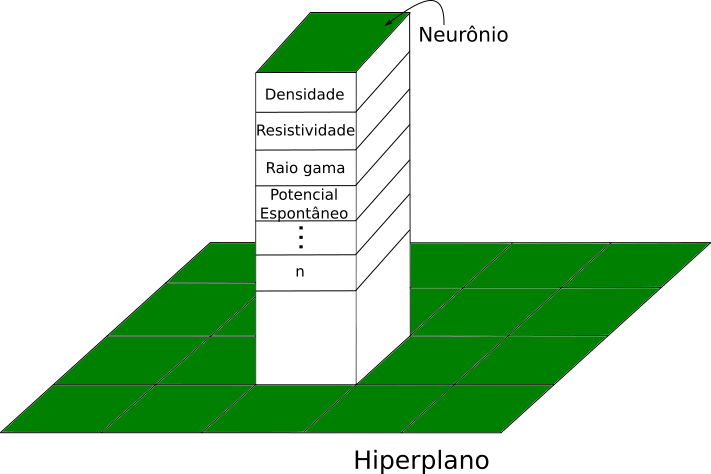
\includegraphics[scale=0.5]{Imagens/hiperplano.png}
	}
	\caption{Neurônio e suas vizinhanças}
	\label{hiperplano}
\end{figure}

O conceito de vizinhança representa uma competição pelo melhor aprendizado e o ajuste do vencedor e da sua vizinhança é um estímulo para que os neurônios ao redor do vencedor também melhorem.

Durante a etapa de treinamento é identificado o neurônio que tem os parâmetros de entrada mais parecidos com os valores dos pesos. Este procedimento é realizado via cálculo da distância euclidiana, Eq. \ref{euclidiana}, entre o parâmetro de entrada $x(t)$ e o peso $w_{i,j}$.

\begin{eqnarray}
d(t)= \sum^{n}_{i=1}[x(t)-w_{i,j}(t)]^{2}
\label{euclidiana}
\end{eqnarray}

A etapa de treinamento da rede se dá por um ajuste de pesos entre os neurônios através do cálculo do menor valor de $d(t)$ na iteração $t$, caracterizando assim o neurônio que passar por esse processo de \textit{vencedor}. Esse procedimento ajusta da mesma forma os pesos do neurônio da vizinhança dentro. Os pesos são ajustados co uma fração da diferença entre os \textit{inputs} $x_{i}$ e os pesos $w_{i}$, vide Eq.\ref{ajuste de pesos}.

\begin{equation}
w_{i,j}(t+1)=w_{i,j}(t)+n(t)[x(t)-w_{i,j}]
\label{ajuste de pesos}
\end{equation}

Através deste ajuste continuado de pesos os elementos do conjunto de entrada são reorganizados de tal foma que as classes próximas sejam posicionados umas perto das outras. Isso gera um mapa bi-dimensional denominado na literatura de \textit{mapa auto-organizável}. Este mapa é o análogo matemático mais fiel das áreas especializadas do córtex cerebral que são ilustradas pelo \textit{Homúnculo de Penfield}, \ref{homunculo}.

\section{Redes com aprendizado não-supervisionado}

Nesta categoria de RNA's são apenas inseridos os valores de \textit{input} da rede. Os \textit{output} são definidos pela própria rede que passa por um processo de treinamento não supervionado. As redes que são submetidas a este tipo de treinamento são mais indicadas para tarefas aonde são exigidos agrupamento de dados (\textit{clustering}). Neste processo uma classe deve ser atribuída aos registros da rede observando-se apenas o comportamento de seus atributos, no caso em particular deste trabalho tratam-se de propriedades geofísicas.

Uma rede com treinamento não supervisionado inspira-se no funcionamento do córtex cerebral. Neste modelo biológico, o organismo aprende a realizar alguma tarefa, por meio da identificação de padrões. Por exemplo, ao identificar uma música determinados padrões sonoros que compõe o conjunto harmonioso de notas precisam ser aprendidos antes de serem reconhecidos. Durante este processo, regiões específicas do cérebro vão sendo paulatinamente acionadas. Isto somente é possível, devido conexões específicas que são formadas entre os neurônios
presentes no córtex, Fig. \ref{homunculo}.

Os detalhes dos processos que regulam o córtex ainda não foram totalmente elucidados, contudo é seguro assumir que a primeira representação dos fenômenos de aprendizagem podem ser representados por uma superfície topológica ou mapa auto-organizado. 

\begin{figure}[H]
	\centering
	\setlength{\fboxsep}{8pt}
	\setlength{\fboxrule}{0.1pt}
	\fbox{
		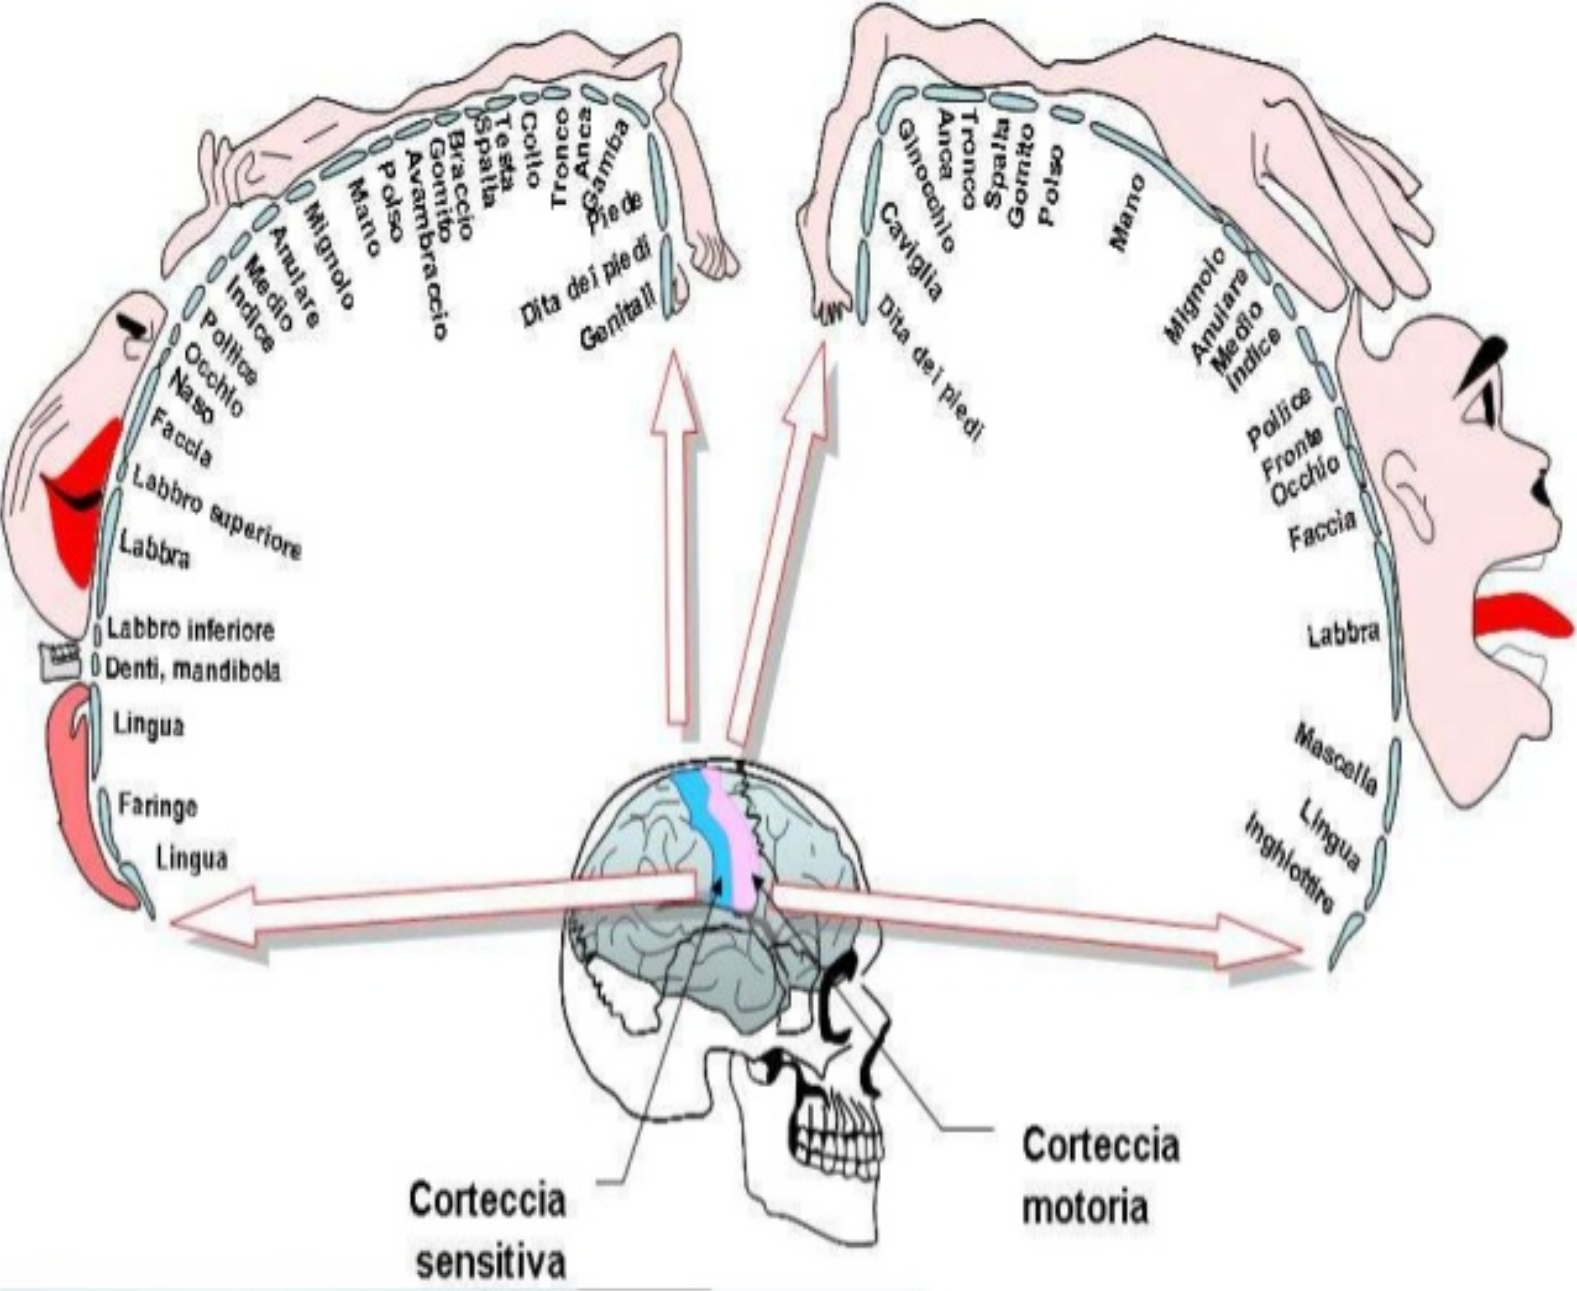
\includegraphics[scale=0.5]{Imagens/homunculo.png}
	}
	\caption{Homúnculo de Penfield.}
	\label{homunculo}
\end{figure}

Um cérebro que sofreu uma comoção grave perde a capacidade de acessar determinadas zonas do homúnculo responsáveis por atividades específicas. Contudo o cérebro tem a capacidade de destinar outras regiões para o controle destas ações que foram previamente perdidas.

Além de casos graves como um acidente o cérebro também perde a capacidade de aprendizado com o tempo. Em humanos, a capacidade de aprendizado vai da pequena infância até a puberdade. Após este período, o cérebro passar a reter o que fora aprendido. Sendo assim o aprendizado é uma função que depende, entre outras coisas, do tempo.

\section{Medidas de Semelhança}

Dado um conjunto de dados numéricos, a \textbf{métrica do dado} é qualquer leitura em uma dada escala de intervalo que infere o grau de diferença entre dois objetos.  Dados que são caracterizados como dados \textbf{não-métricos}, são aqueles conjuntos de dados que podem ser coletados em um formato \textit{binário} (0/1),  \textit{ordinário} números que expressam uma posição somente (índice), ou \textit{escala nominal} que são conjuntos de dados não ordenados \citep{Michel2016}.

Na análise geométrica do dado se refere aos aspectos geométricos da imagem, análise de padrões ou forma, que trata um conjunto arbitrário de dados como uma nuvem de pontos no espaço  $\Re ^{n}$. O dado passa a ser organizado em uma base de dados indexadas em um espaço métrico\footnote{Este processo é conhecido como indexação métrica.}.

Na análise de agrupamentos (classificação, taxonomia, reconhecimento de padrões) consiste em dividir o dado $A$ em um conjunto menor de grupos. Por exemplo, um grupo de dados que estão próximos em respeito a um determinado critério como propriedades físicas em rochas. 

Neste trabalho são estudadas duas medidas de semelhança especiais. A primeira delas e a métrica de \textit{Euclides} que leva em consideração o cálculo de centroides para avaliar a distância entre dois agrupamentos. A segunda é a métrica de \textit{Mahalanobis} que leva em consideração a forma do agrupamento a ser analisado.   

\subsection{A métrica Euclideana}

Dado dois conjuntos de agrupamentos distintos, $\theta$($\bar{x}_{i},\bar{y}_{i}$) e $\beta$($\bar{x}_{j},\bar{y}_{j}$), os seus vetores de coordenadas cartesianas podem ser definidos como

\begin{multicols}{2}
	\begin{equation}
	 \textbf{x}^{i}=
		\begin{bmatrix} 
		x_{1}^{i} \\
		x_{2}^{i} \\
		x_{2}^{i} \\
		\vdots \\
		x_{m}^{i}
		\end{bmatrix}
	\end{equation}
	
   \begin{equation}
      \textbf{y}^{i}=
    	\begin{bmatrix} 
       	y_{1}^{i} \\
    	y_{2}^{i} \\
    	y_{2}^{i} \\
	     \vdots \\
	    y_{m}^{i}
    	\end{bmatrix}
   \end{equation}
\end{multicols}

para um agrupamento $\theta$, e 

\begin{multicols}{2}

\begin{equation}
     \textbf{x}^{j}=
		\begin{bmatrix} 
		x_{1}^{j} \\
		x_{2}^{j} \\
		x_{2}^{j} \\
		\vdots \\
		x_{n}^{j}
		\end{bmatrix}
\end{equation}

\begin{equation}
      \textbf{y}^{j}=
		\begin{bmatrix} 
		y_{1}^{j} \\
		y_{2}^{j} \\
		y_{2}^{j} \\
		\vdots \\
		y_{n}^{j}
		\end{bmatrix}
\end{equation}
\end{multicols}

para outro agrupamento  $\beta$.  A métrica euclideana, na sua forma mais genérica, pode ser definida como uma distância ponderada, de acordo com a Eq. \ref{eucli}.

\begin{equation}
[(\bar{\textbf{x}_{i}}-\bar{\textbf{x}}_{j})^{T}\textbf{A}(\bar{\textbf{y}}_{i}-\bar{\textbf{y}}_{j})]^{1/2}
\label{eucli}
\end{equation}

Onde $\textbf{A}$ é uma matriz não-singular e simétrica de dimensão $m \times n $ e com $m=n$, $\bar{\textbf{x}}_{i}$ é a média do vetor de coordenadas cartesianas do agrupamento $\theta$ com dimensão $m$, $\bar{\text{y}}_{i}$ é a média do segundo vetor de coordenadas do agrupamento $\theta$ com dimensão $m$, $\bar{\textbf{x}}_{j}$ é a média do vetor de coordenadas do agrupamento $\beta$ com dimensão $n$, $\bar{\textbf{y}}_{j}$ é a média do segundo vetor de coordenadas cartesianas do agrupamento $\beta$ também com dimensão $n$.

Nos casos em que $\textbf{A} = \textbf{I}$, onde $\textbf{I}$ é a matriz identidade obtém-se a métrica euclideana não-ponderada, que é o caso estudado neste trabalho. 

A métrica euclideana é de fácil compreensão. Contudo sua utilização apenas apresenta bons resultados, quando todas as classes possuam a mesma variância. Além disso, os elementos dos vetores não devem possuir nenhum tipo de correlação entre si, em resumo, estes devem ser circulares. E no espaço de propriedades, onde os elementos dos vetores se distribuem, isso raramente ocorre. 

\subsection{A métrica de Mahalanobis}

A distância de Mahalanobis é um caso particular da métrica euclideana onde, no lugar da matriz $\textbf{A}$, utiliza-se a matriz de covariância agrupada inversa $\textbf{S}$. Esta métrica mede a separação entre dois grupos de objetos levando-se em consideração o formato da distribuição dos dados. Suponhamos que nós tenhamos dois grupos de objetos com médias $\bar{\textbf{x}}_{i}$ e $\bar{\textbf{x}}_{j}$, a distância de Mahalanobis é dado pelo seguinte enunciado, Eq. \ref{maha}:

\begin{equation}
[(\bar{\textbf{x}_{i}}-\bar{\textbf{x}}_{j})^{T}\textbf{S}^{-1}(\bar{\textbf{y}}_{i}-\bar{\textbf{y}}_{j})]^{1/2}
\label{maha}
\end{equation}

Os dados dos dois grupos devem ter o mesmo número de variáveis (o mesmo número de colunas), mas não necessariamente o mesmo número de dados (cada grupo pode possuir diferentes número de linhas). A matriz covariância para o grupo $i$ é calculada usando uma matriz de dados centralizada $\hat{\textbf{X}}$.


\begin{equation}
\textbf{C}_{i}=\dfrac{1}{n} \hat{\textbf{X}_{i}}^{T}\hat{\textbf{X}_{i}}
\end{equation}

Onde $n=\sum_{i} n_{i}$, ou seja a soma de todos os dados de todos os grupos. 


A matriz de covariância agrupada $\textbf{S}$ (\textit{Pooled Covariance Matrix}) dos dois agrupamentos ($\theta, \beta$) é computada como a média ponderada das matrizes de covariância:

\begin{equation}
\textbf{S}(\theta, \beta)=\dfrac{1}{n}\sum^{g}_{i=1}n_{i}C_{i}
\end{equation}

Onde $\theta$ e $\beta$ representam os dois agrupamentos e $g$ é o número de agrupamentos.


\subsection{Análise de agrupamento}
\label{teste}

Ao se criar uma análise de agrupamentos tem-se em vista a caracterização do quão semelhante, ou não, dois ou mais conjuntos de dados podem ser.  Para se determinar em qual situação cada métrica se comporta melhor, foi gerado um teste analítico com vistas a se comparar tanto a distância quanto a forma da distribuição dos dados influem no valor absoluto final das duas métricas. 

No primeiro teste, gerou-se distribuições randômicas circulares de três agrupamentos com seus centros igualmente espaçados como apresentado na Fig. \ref{AC1}. Nota-se que os clusters encontram-se a $20$ unidades de distância entre seus respectivos centros. 

\begin{figure}[H]
	\centering
	\setlength{\fboxsep}{8pt}
	\setlength{\fboxrule}{0.1pt}
	\fbox{
		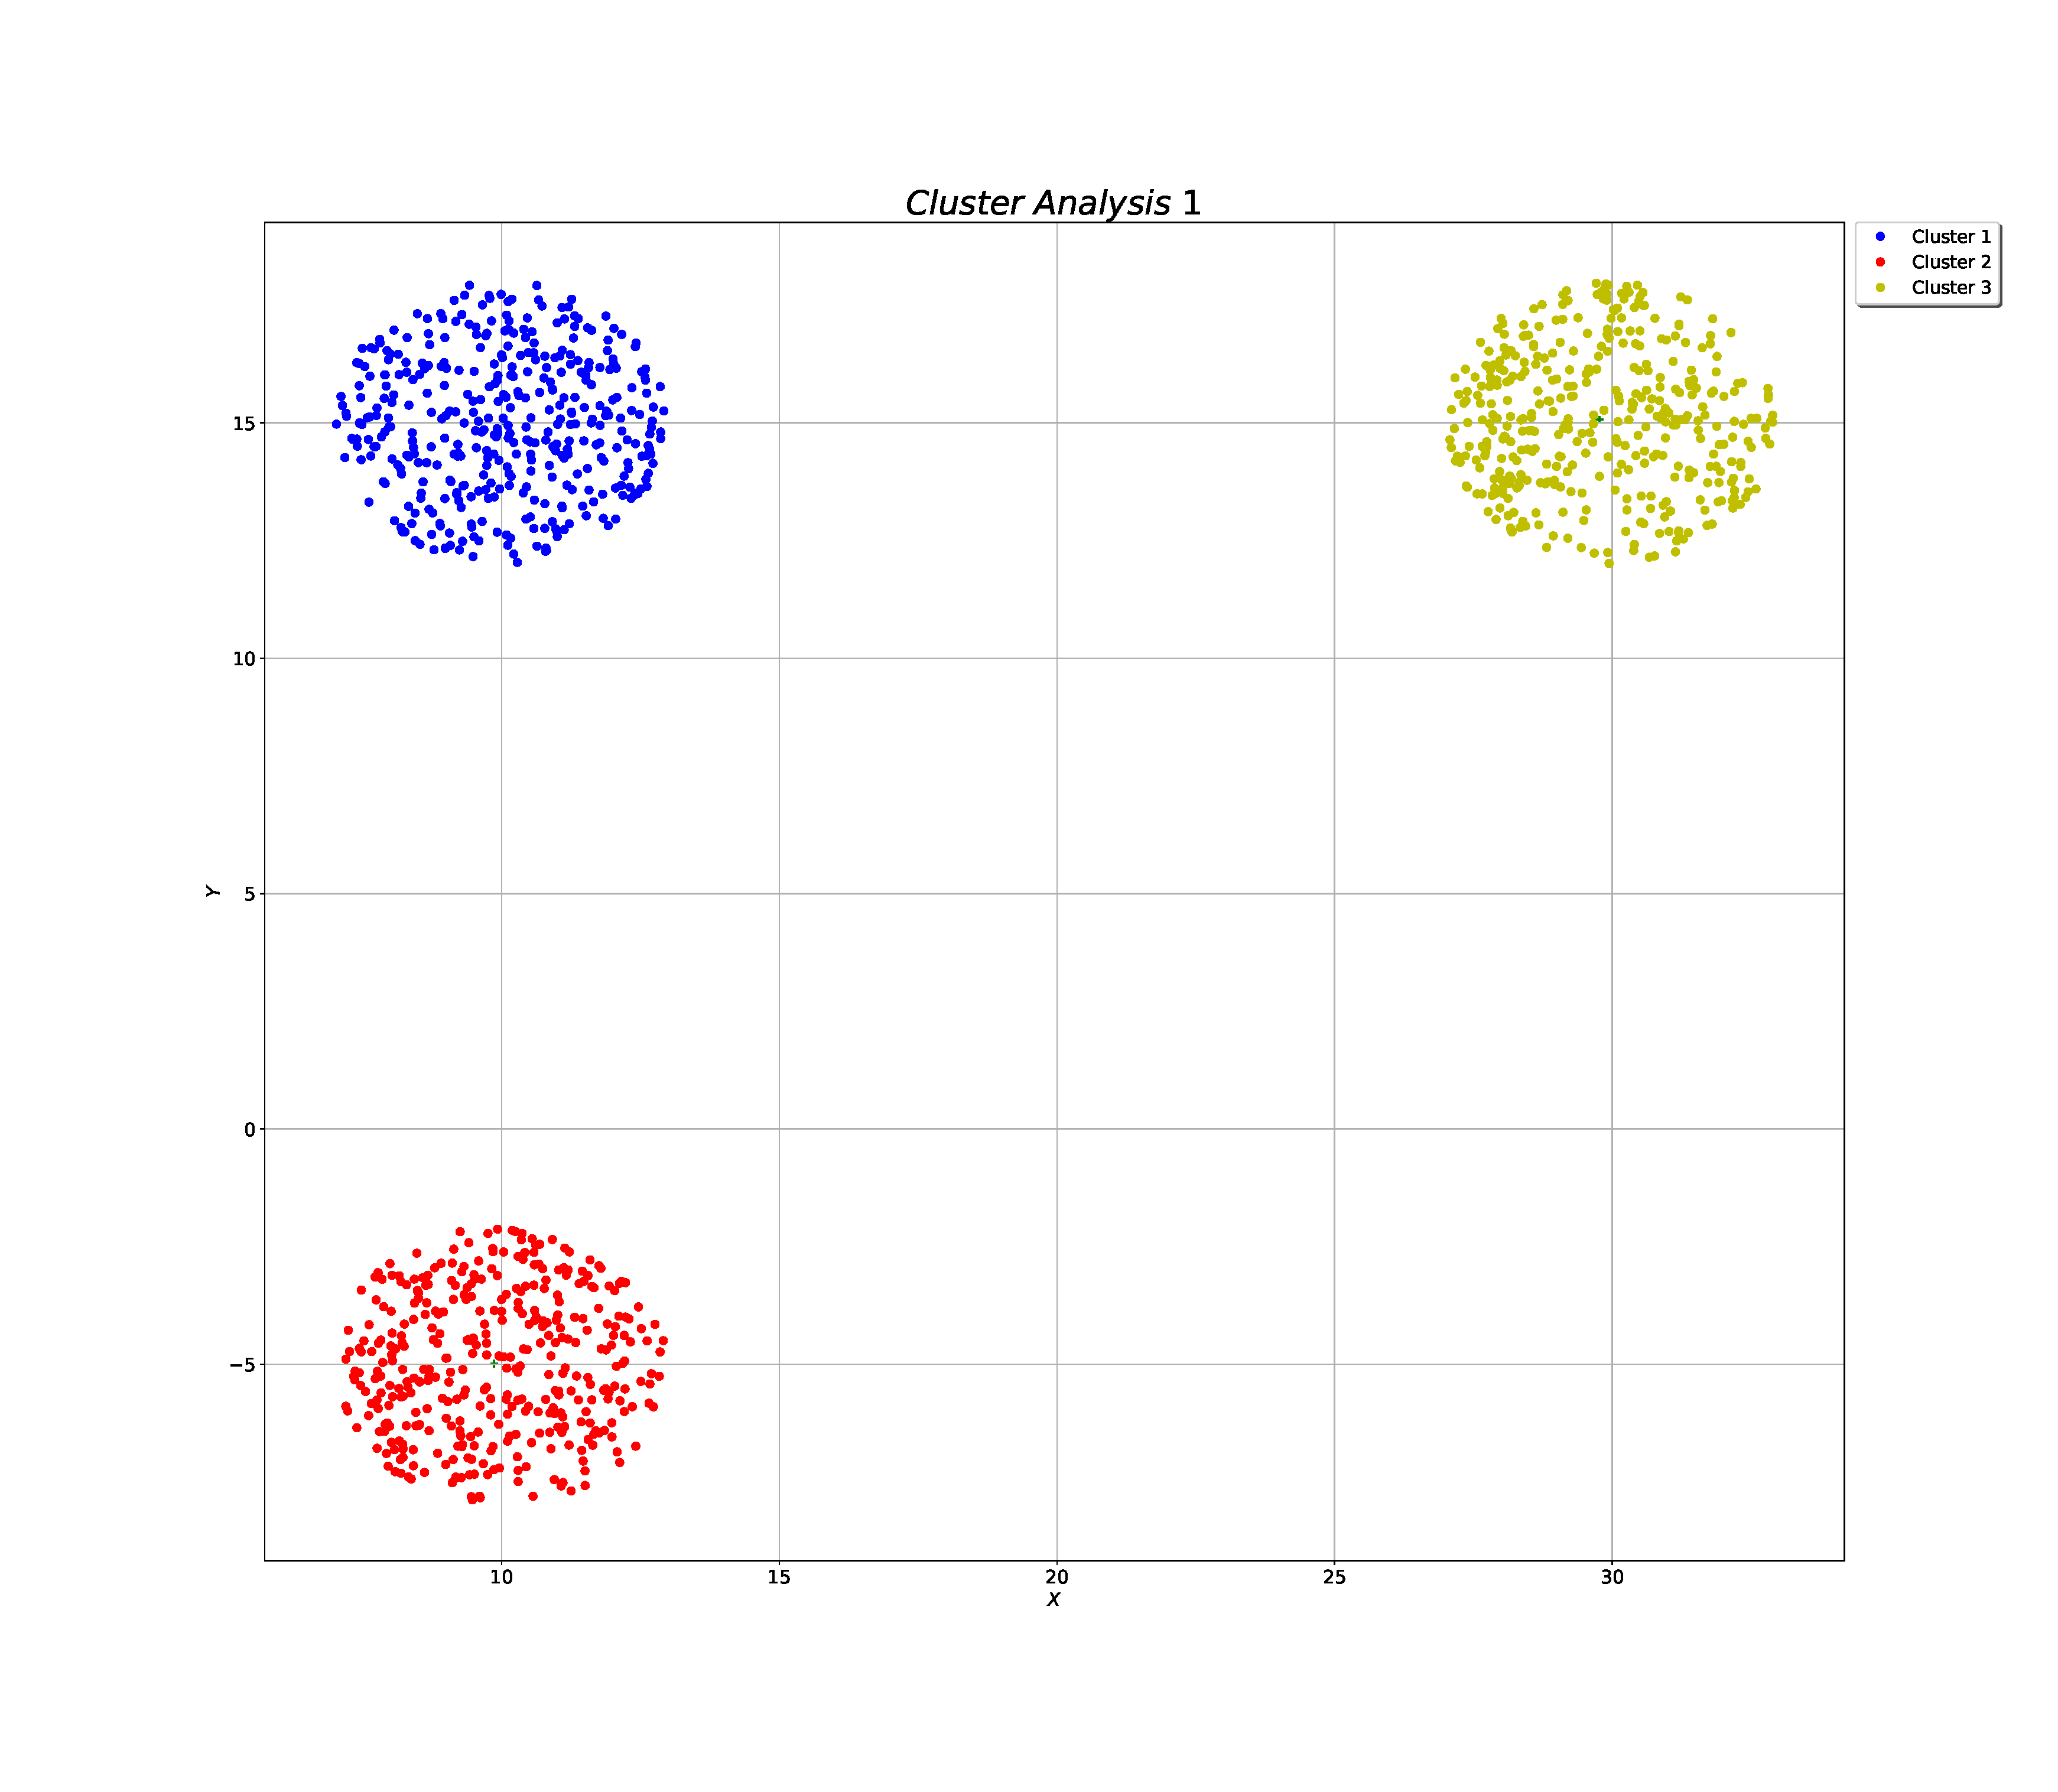
\includegraphics[scale=0.20]{Imagens/clusteranalise1.eps}
	}
	\caption{Análise de agrupamento 1}
	\label{AC1}
\end{figure}

O primeiro caso estudado apresentam três circunferências compostas por diferentes conjuntos de dados. Os parâmetros utilizados para criar a primeira situação de estudo são apresentadas na Tab. \ref{analise1}.

\begin{table}[H]
	\centering
	\caption{Parâmetros dos teste analítico para comparação das métricas.}
	\label{analise1}
	\begin{tabular}{lccc}
		\hline
		Parâmetros       & \textcolor{blue}{Cluster1} & \textcolor{red}{Cluster 2} & \textcolor{olive}{Cluster 3} \\ \hline
		Raio máximo      & 0.300E+01 & 0.300E+01 & 0.300E+01 \\
		Raio mínimo      & 0.000E+00 & 0.000E+00 & 0.000E+00 \\
		Ângulo máximo    & 0.157E+02 & 0.157E+02 & 0.157E+02 \\
		Ângulo mínimo    & 0.000E+00 & 0.000E+00 & 0.000E+00 \\
		Semente                & 5                 & 5                  & 5         \\
		Número de pontos & 404       & 383       & 397   \\        \hline
	\end{tabular}
\end{table}

Para os casos em que a distribuição, no espaço de propriedades, apresenta simetria em ambos os eixos as métricas apresentam uma pequena diferença entre si. A distância de Euclides medida entre os agrumamentos I e II foi de $20,0$ unidades de medida, enquanto que a mesma distância medida entre os clusters I-III foi de $19,8$ unidades de medida. Tal diferença se deve a imprecisão associada ao sorteio randômico e o deslocamento dos centros das distribuições. 

A distância de Mahalanobis leva em consideração a forma das distribuições de dados ao longo do espaço de propriedades.  O resultado desta métrica para os agrupamentos I-II foi de $13,8$, enquanto que a mesma métrica para os agrupamentos I-III foi de $12,9$. Mostrando que os resultados se afastam um pouco mais.
 
 \begin{table}[H]
 	\centering
 	\label{metrica1}
 	\begin{tabular}{|l|l|}
 		\hline
 		\multicolumn{2}{|c|}{Distâncias}  \\ \hline
 		Euclideana (I-II)     & 0.200E+02 \\ \hline
 		Mahalanobeana (I-II)  & 0.138E+02 \\ \hline
 		Euclideana (I-III)    & 0.197E+02 \\ \hline
 		Mahalanobeana (I-III) & 0.129E+02 \\ \hline
 	\end{tabular}
 \end{table}


O segundo teste apresenta uma leve deformação no agrupamento I (em \textcolor{blue}{azul}), Fig. \ref{AC2}.  Um pequeno aumento do eixo horizontal muda a distribuição para uma forma levemente elipsoidal de dados no espaço. Os demais clusters continuam com uma distribuição circular.



\begin{figure}[H]
	\centering
	\setlength{\fboxsep}{8pt}
	\setlength{\fboxrule}{0.1pt}
	\fbox{
		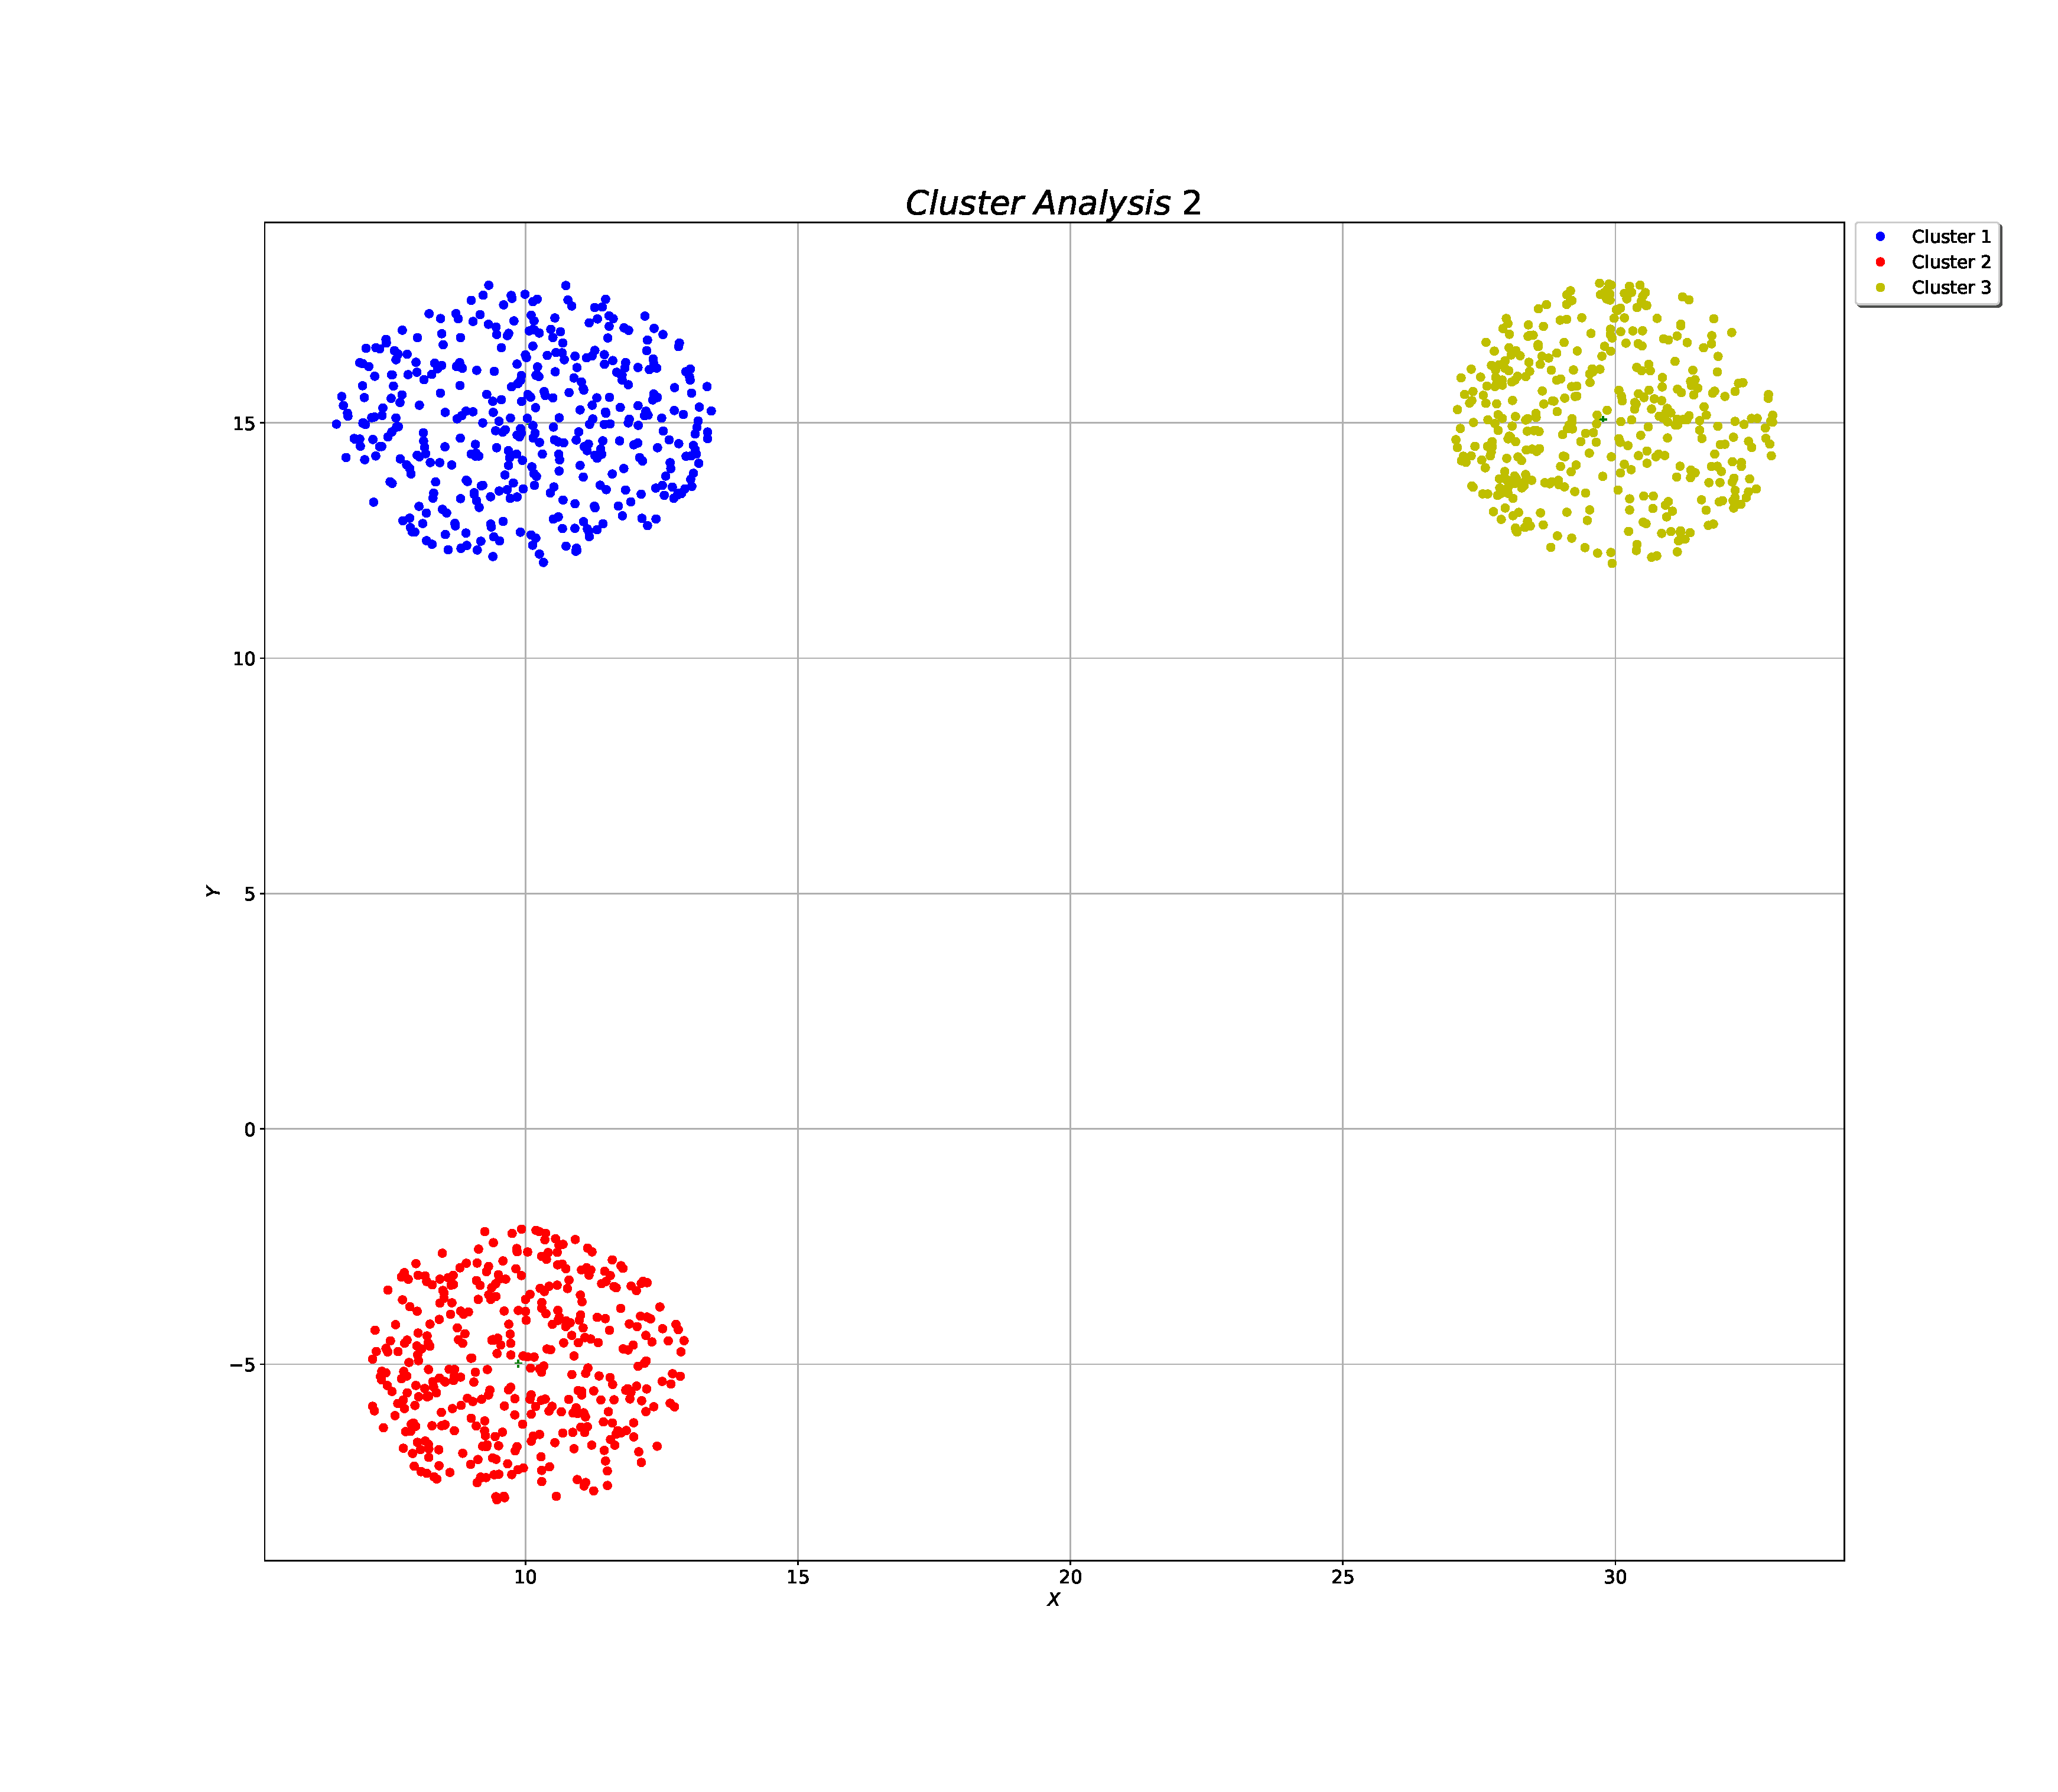
\includegraphics[scale=0.20]{Imagens/clusteranalise2.eps}
	}
	\caption{Análise de agrupamento 2}
	\label{AC2}
\end{figure}

A Tab. \ref{analise2} mostram os parâmetros utilizados para a criação de cada um dos clusters. Salienta-se a principal mudança foi um leve aumento do eixo horizontal da ordem de $0,5$ unidades de medida. Os demais parâmetros tais como posição e número de dados dos clusters permaneceram inalterados. 

\begin{table}[H]
	\centering
	\caption{Parâmetros do segundo teste analítico.}
	\label{analise2}
	\begin{tabular}{lccc}
		\hline
		Parâmetros       & \textcolor{blue}{Cluster1} & \textcolor{red}{Cluster 2} & \textcolor{olive}{Cluster 3} \\ \hline
		Raio máximo      & --- & 0.300E+01 & 0.300E+01 \\
		Raio mínimo      & --- & 0.000E+00 & 0.000E+00 \\
		Ângulo máximo    & 0.157E+02 & 0.157E+02 & 0.157E+02 \\
		Ângulo mínimo    & 0.000E+00 & 0.000E+00 & 0.000E+00 \\
		Eixo maior        & 0.350E+01        & ----         & ---         \\
		Eixo menor          & 0.300E+01        & ---       & ---        \\
		Semente          & 9         & 9         & 9         \\
		Número de pontos & 405       & 383       & 396   \\   \hline
	\end{tabular}
\end{table}

No segundo caso, a distância de Euclides permaneceu inalterada para ambos os casos, tanto na distância entre os agrupamentos I-II e I-III. Isso se deve ao fato de os centroides permanecerem inalterados para as análises de agrupamentos 1 e 2, observando-se um valor de $20,0$ e $19,7$ unidades de distância. 
A distância de Mahalanobis sofreu o maior impacto no seu valor absoluto, na ordem de $2$ unidades de medida entre os agrupamentos I-III. De maneira geral os padrões de comportamento das métricas permaneceram inalterados, com exceção do caso aonde a Mahalanobis foi de $11,8$ unidades de medida demonstrando a sensibilidade esperada para deformações em grupos de dados. Enquanto que o valor encontrado para o agrupamento I-II foi de $13,8$, muito semelhante ao do teste anterior. 

 \begin{table}[H]
 	\centering
 	\label{metrica2}
 	\begin{tabular}{|l|l|}
 		\hline
 		\multicolumn{2}{|c|}{Distâncias}  \\ \hline
 		Euclideana (I-II)     & 0.200E+02 \\ \hline
 		Mahalanobeana (I-II)  & 0.138E+02 \\ \hline
 		Euclideana (I-III)    & 0.197E+02 \\ \hline
 		Mahalanobeana (I-III) &  0.118E+02 \\ \hline
 	\end{tabular}
 \end{table}


O terceiro teste apresenta o agrupamento 1 com um formato elipsoidal oblato se aproximando mais do agrupamento 3. Este comportamento é retratado na Fig. \ref{AC3}. Os demais conjuntos de agrupamentos permaneceram com a mesma forma dos testes anteriores. 

\begin{figure}[H]
	\centering
	\setlength{\fboxsep}{8pt}
	\setlength{\fboxrule}{0.1pt}
	\fbox{
		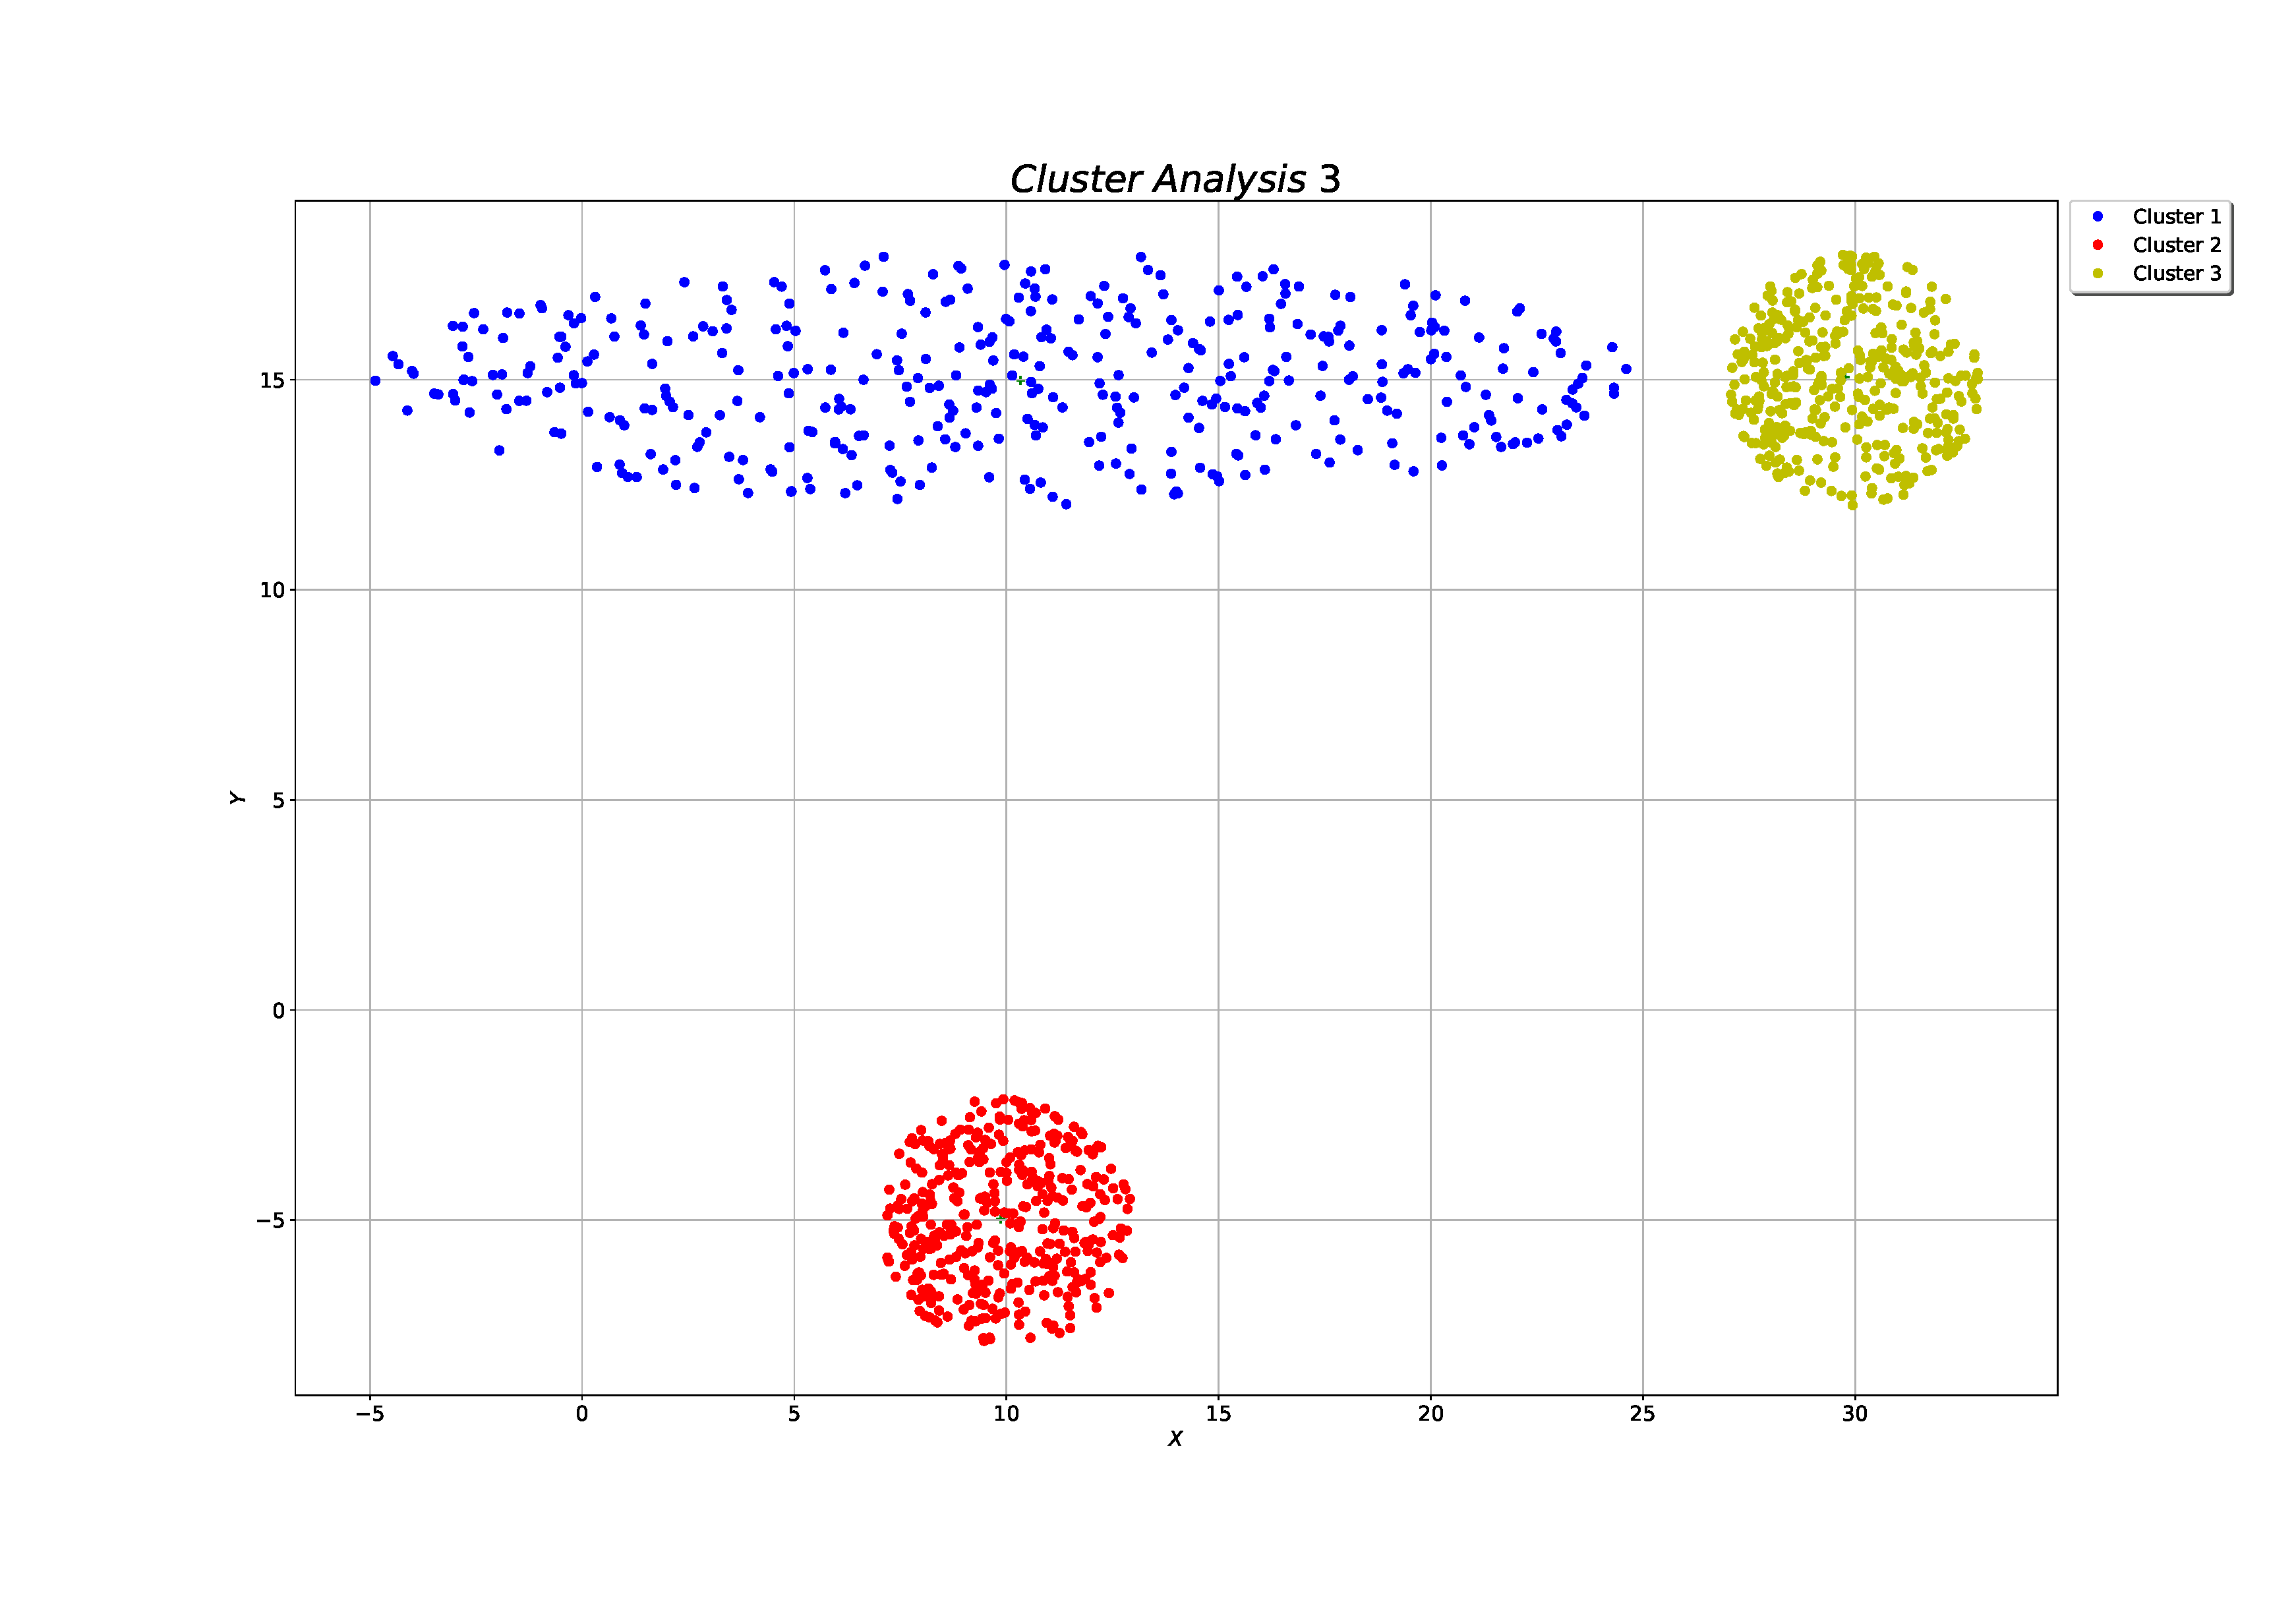
\includegraphics[scale=0.25]{Imagens/clusteranalise3.eps}
	}
	\caption{Análise de agrupamento 3}
	\label{AC3}
\end{figure}


A deformação explícita no agrupamento 1 se deu por conta do aumento de $11,5$ unidades de medida do eixo horizontal. Essa perturbação na forma da elipse em contraste com os demais clusters é descrita na Tab. \ref{analise3}.


\begin{table}[H]
	\centering
	\caption{Parâmetros dos teste analítico para comparação das métricas.}
	\label{analise3}
	\begin{tabular}{lccc}
		\hline
		Parâmetros       & \textcolor{blue}{Cluster1} & \textcolor{red}{Cluster 2} & \textcolor{olive}{Cluster 3} \\ \hline
		Raio máximo      & --- & 0.300E+01 & 0.300E+01 \\
		Raio mínimo      & --- & 0.000E+00 & 0.000E+00 \\
		Ângulo máximo    & 0.157E+02 & 0.157E+02 & 0.157E+02 \\
		Ângulo mínimo    & 0.000E+00 & 0.000E+00 & 0.000E+00 \\
		Eixo maior        & 0.150E+02        & ----         & ---         \\
		Eixo menor          &  0.300E+01        & ---       & ---        \\
		Semente          & 17         & 17         & 17         \\
		Número de pontos & 405       & 384       & 395  \\   \hline
	\end{tabular}
\end{table}


 \begin{table}[H]
 	\centering
 	\label{metrica3}
 	\begin{tabular}{|l|l|}
 		\hline
 		\multicolumn{2}{|c|}{Distâncias}  \\ \hline
 		Euclideana (I-II)     & 0.200E+02 \\ \hline
 		Mahalanobeana (I-II)  & 0.138E+02 \\ \hline
 		Euclideana (I-III)    & 0.194E+02 \\ \hline
 		Mahalanobeana (I-III) & 0.352E+01 \\ \hline
 	\end{tabular}
 \end{table}

A distância de Euclides permaneceu inalterada dos três casos estudados entre os três agrupamentos. Apresentando o valor de $2,0$ e $19,4$ para as distâncias entre os agrupamentos I-II e I-III respectivamente. Contudo, o cômputo da distância de Mahalanobis apresentou uma grande diferença se comparado as análises anteriores. Apresentando o valor de $13,8$ unidades de medida entre os agrupamentos I-II e $3,5$ unidades de medida entre os agrupamentos I-III.  

Esta pequena análise demonstra que o cômputo da distância de Mahalanobis está intimamente relacionada com a forma da distribuição dos dados dentro do espaço de propriedades quando comparada a distância Euclideana. Isto se deve ao cálculo da matriz de covariância para cada classe de dados \ref{maha}, que permite levar em conta a forma do agrupamento em questão. 


